\documentclass[1p]{elsarticle_modified}
%\bibliographystyle{elsarticle-num}

%\usepackage[colorlinks]{hyperref}
%\usepackage{abbrmath_seonhwa} %\Abb, \Ascr, \Acal ,\Abf, \Afrak
\usepackage{amsfonts}
\usepackage{amssymb}
\usepackage{amsmath}
\usepackage{amsthm}
\usepackage{scalefnt}
\usepackage{amsbsy}
\usepackage{kotex}
\usepackage{caption}
\usepackage{subfig}
\usepackage{color}
\usepackage{graphicx}
\usepackage{xcolor} %% white, black, red, green, blue, cyan, magenta, yellow
\usepackage{float}
\usepackage{setspace}
\usepackage{hyperref}

\usepackage{tikz}
\usetikzlibrary{arrows}

\usepackage{multirow}
\usepackage{array} % fixed length table
\usepackage{hhline}

%%%%%%%%%%%%%%%%%%%%%
\makeatletter
\renewcommand*\env@matrix[1][\arraystretch]{%
	\edef\arraystretch{#1}%
	\hskip -\arraycolsep
	\let\@ifnextchar\new@ifnextchar
	\array{*\c@MaxMatrixCols c}}
\makeatother %https://tex.stackexchange.com/questions/14071/how-can-i-increase-the-line-spacing-in-a-matrix
%%%%%%%%%%%%%%%

\usepackage[normalem]{ulem}

\newcommand{\msout}[1]{\ifmmode\text{\sout{\ensuremath{#1}}}\else\sout{#1}\fi}
%SOURCE: \msout is \stkout macro in https://tex.stackexchange.com/questions/20609/strikeout-in-math-mode

\newcommand{\cancel}[1]{
	\ifmmode
	{\color{red}\msout{#1}}
	\else
	{\color{red}\sout{#1}}
	\fi
}

\newcommand{\add}[1]{
	{\color{blue}\uwave{#1}}
}

\newcommand{\replace}[2]{
	\ifmmode
	{\color{red}\msout{#1}}{\color{blue}\uwave{#2}}
	\else
	{\color{red}\sout{#1}}{\color{blue}\uwave{#2}}
	\fi
}

\newcommand{\Sol}{\mathcal{S}} %segment
\newcommand{\D}{D} %diagram
\newcommand{\A}{\mathcal{A}} %arc


%%%%%%%%%%%%%%%%%%%%%%%%%%%%%5 test

\def\sl{\operatorname{\textup{SL}}(2,\Cbb)}
\def\psl{\operatorname{\textup{PSL}}(2,\Cbb)}
\def\quan{\mkern 1mu \triangleright \mkern 1mu}

\theoremstyle{definition}
\newtheorem{thm}{Theorem}[section]
\newtheorem{prop}[thm]{Proposition}
\newtheorem{lem}[thm]{Lemma}
\newtheorem{ques}[thm]{Question}
\newtheorem{cor}[thm]{Corollary}
\newtheorem{defn}[thm]{Definition}
\newtheorem{exam}[thm]{Example}
\newtheorem{rmk}[thm]{Remark}
\newtheorem{alg}[thm]{Algorithm}

\newcommand{\I}{\sqrt{-1}}
\begin{document}

%\begin{frontmatter}
%
%\title{Boundary parabolic representations of knots up to 8 crossings}
%
%%% Group authors per affiliation:
%\author{Yunhi Cho} 
%\address{Department of Mathematics, University of Seoul, Seoul, Korea}
%\ead{yhcho@uos.ac.kr}
%
%
%\author{Seonhwa Kim} %\fnref{s_kim}}
%\address{Center for Geometry and Physics, Institute for Basic Science, Pohang, 37673, Korea}
%\ead{ryeona17@ibs.re.kr}
%
%\author{Hyuk Kim}
%\address{Department of Mathematical Sciences, Seoul National University, Seoul 08826, Korea}
%\ead{hyukkim@snu.ac.kr}
%
%\author{Seokbeom Yoon}
%\address{Department of Mathematical Sciences, Seoul National University, Seoul, 08826,  Korea}
%\ead{sbyoon15@snu.ac.kr}
%
%\begin{abstract}
%We find all boundary parabolic representation of knots up to 8 crossings.
%
%\end{abstract}
%\begin{keyword}
%    \MSC[2010] 57M25 
%\end{keyword}
%
%\end{frontmatter}

%\linenumbers
%\tableofcontents
%
\newcommand\colored[1]{\textcolor{white}{\rule[-0.35ex]{0.8em}{1.4ex}}\kern-0.8em\color{red} #1}%
%\newcommand\colored[1]{\textcolor{white}{ #1}\kern-2.17ex	\textcolor{white}{ #1}\kern-1.81ex	\textcolor{white}{ #1}\kern-2.15ex\color{red}#1	}

{\Large $\underline{12n_{0191}~(K12n_{0191})}$}

\setlength{\tabcolsep}{10pt}
\renewcommand{\arraystretch}{1.6}
\vspace{1cm}\begin{tabular}{m{100pt}>{\centering\arraybackslash}m{274pt}}
\multirow{5}{120pt}{
	\centering
	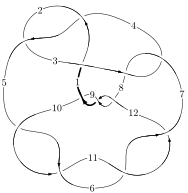
\includegraphics[width=112pt]{../../../GIT/diagram.site/Diagrams/png/2280_12n_0191.png}\\
\ \ \ A knot diagram\footnotemark}&
\allowdisplaybreaks
\textbf{Linearized knot diagam} \\
\cline{2-2}
 &
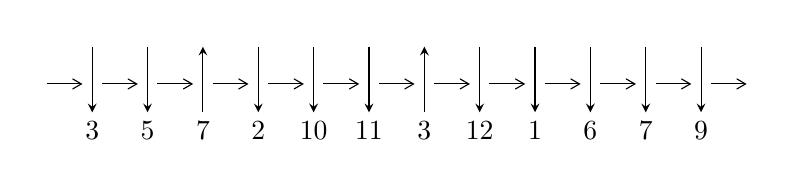
\begin{tikzpicture}[x=20pt, y=17pt]
	% nodes
	\node (C0) at (0, 0) {};
	\node (C1) at (1, 0) {};
	\node (C1U) at (1, +1) {};
	\node (C1D) at (1, -1) {3};

	\node (C2) at (2, 0) {};
	\node (C2U) at (2, +1) {};
	\node (C2D) at (2, -1) {5};

	\node (C3) at (3, 0) {};
	\node (C3U) at (3, +1) {};
	\node (C3D) at (3, -1) {7};

	\node (C4) at (4, 0) {};
	\node (C4U) at (4, +1) {};
	\node (C4D) at (4, -1) {2};

	\node (C5) at (5, 0) {};
	\node (C5U) at (5, +1) {};
	\node (C5D) at (5, -1) {10};

	\node (C6) at (6, 0) {};
	\node (C6U) at (6, +1) {};
	\node (C6D) at (6, -1) {11};

	\node (C7) at (7, 0) {};
	\node (C7U) at (7, +1) {};
	\node (C7D) at (7, -1) {3};

	\node (C8) at (8, 0) {};
	\node (C8U) at (8, +1) {};
	\node (C8D) at (8, -1) {12};

	\node (C9) at (9, 0) {};
	\node (C9U) at (9, +1) {};
	\node (C9D) at (9, -1) {1};

	\node (C10) at (10, 0) {};
	\node (C10U) at (10, +1) {};
	\node (C10D) at (10, -1) {6};

	\node (C11) at (11, 0) {};
	\node (C11U) at (11, +1) {};
	\node (C11D) at (11, -1) {7};

	\node (C12) at (12, 0) {};
	\node (C12U) at (12, +1) {};
	\node (C12D) at (12, -1) {9};
	\node (C13) at (13, 0) {};

	% arrows
	\draw[->,>={angle 60}]
	(C0) edge (C1) (C1) edge (C2) (C2) edge (C3) (C3) edge (C4) (C4) edge (C5) (C5) edge (C6) (C6) edge (C7) (C7) edge (C8) (C8) edge (C9) (C9) edge (C10) (C10) edge (C11) (C11) edge (C12) (C12) edge (C13) ;	\draw[->,>=stealth]
	(C1U) edge (C1D) (C2U) edge (C2D) (C3D) edge (C3U) (C4U) edge (C4D) (C5U) edge (C5D) (C6U) edge (C6D) (C7D) edge (C7U) (C8U) edge (C8D) (C9U) edge (C9D) (C10U) edge (C10D) (C11U) edge (C11D) (C12U) edge (C12D) ;
	\end{tikzpicture} \\
\hhline{~~} \\& 
\textbf{Solving Sequence} \\ \cline{2-2} 
 &
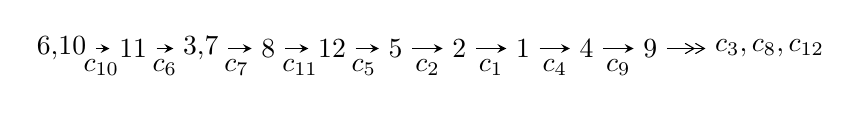
\begin{tikzpicture}[x=23pt, y=7pt]
	% node
	\node (A0) at (-1/8, 0) {6,10};
	\node (A1) at (1, 0) {11};
	\node (A2) at (33/16, 0) {3,7};
	\node (A3) at (25/8, 0) {8};
	\node (A4) at (33/8, 0) {12};
	\node (A5) at (41/8, 0) {5};
	\node (A6) at (49/8, 0) {2};
	\node (A7) at (57/8, 0) {1};
	\node (A8) at (65/8, 0) {4};
	\node (A9) at (73/8, 0) {9};
	\node (C1) at (1/2, -1) {$c_{10}$};
	\node (C2) at (3/2, -1) {$c_{6}$};
	\node (C3) at (21/8, -1) {$c_{7}$};
	\node (C4) at (29/8, -1) {$c_{11}$};
	\node (C5) at (37/8, -1) {$c_{5}$};
	\node (C6) at (45/8, -1) {$c_{2}$};
	\node (C7) at (53/8, -1) {$c_{1}$};
	\node (C8) at (61/8, -1) {$c_{4}$};
	\node (C9) at (69/8, -1) {$c_{9}$};
	\node (A10) at (11, 0) {$c_{3},c_{8},c_{12}$};

	% edge
	\draw[->,>=stealth]	
	(A0) edge (A1) (A1) edge (A2) (A2) edge (A3) (A3) edge (A4) (A4) edge (A5) (A5) edge (A6) (A6) edge (A7) (A7) edge (A8) (A8) edge (A9) ;
	\draw[->>,>={angle 60}]	
	(A9) edge (A10);
\end{tikzpicture} \\ 

\end{tabular} \\

\footnotetext{
The image of knot diagram is generated by the software ``\textbf{Draw programme}" developed by Andrew Bartholomew(\url{http://www.layer8.co.uk/maths/draw/index.htm\#Running-draw}), where we modified some parts for our purpose(\url{https://github.com/CATsTAILs/LinksPainter}).
}\phantom \\ \newline 
\centering \textbf{Ideals for irreducible components\footnotemark of $X_{\text{par}}$} 
 
\begin{align*}
I^u_{1}&=\langle 
2.93013\times10^{22} u^{41}-2.55618\times10^{22} u^{40}+\cdots+3.19018\times10^{22} b+3.37541\times10^{22},\\
\phantom{I^u_{1}}&\phantom{= \langle  }3.37341\times10^{22} u^{41}-5.52290\times10^{22} u^{40}+\cdots+3.19018\times10^{22} a-5.34100\times10^{22},\;u^{42}-2 u^{41}+\cdots+9 u^2-1\rangle \\
I^u_{2}&=\langle 
b-1,\;- u^2+a- u+1,\;u^3+u^2-2 u-1\rangle \\
\\
\end{align*}
\raggedright * 2 irreducible components of $\dim_{\mathbb{C}}=0$, with total 45 representations.\\
\footnotetext{All coefficients of polynomials are rational numbers. But the coefficients are sometimes approximated in decimal forms when there is not enough margin.}
\newpage
\renewcommand{\arraystretch}{1}
\centering \section*{I. $I^u_{1}= \langle 2.93\times10^{22} u^{41}-2.56\times10^{22} u^{40}+\cdots+3.19\times10^{22} b+3.38\times10^{22},\;3.37\times10^{22} u^{41}-5.52\times10^{22} u^{40}+\cdots+3.19\times10^{22} a-5.34\times10^{22},\;u^{42}-2 u^{41}+\cdots+9 u^2-1 \rangle$}
\flushleft \textbf{(i) Arc colorings}\\
\begin{tabular}{m{7pt} m{180pt} m{7pt} m{180pt} }
\flushright $a_{6}=$&$\begin{pmatrix}0\\u\end{pmatrix}$ \\
\flushright $a_{10}=$&$\begin{pmatrix}1\\0\end{pmatrix}$ \\
\flushright $a_{11}=$&$\begin{pmatrix}1\\u^2\end{pmatrix}$ \\
\flushright $a_{3}=$&$\begin{pmatrix}-1.05743 u^{41}+1.73122 u^{40}+\cdots+2.10719 u+1.67420\\-0.918482 u^{41}+0.801265 u^{40}+\cdots-1.32965 u-1.05806\end{pmatrix}$ \\
\flushright $a_{7}=$&$\begin{pmatrix}- u\\- u^3+u\end{pmatrix}$ \\
\flushright $a_{8}=$&$\begin{pmatrix}-0.468740 u^{41}+1.75288 u^{40}+\cdots-2.79645 u+2.00796\\0.403032 u^{41}-0.477459 u^{40}+\cdots-0.178275 u-0.123472\end{pmatrix}$ \\
\flushright $a_{12}=$&$\begin{pmatrix}- u^2+1\\- u^4+2 u^2\end{pmatrix}$ \\
\flushright $a_{5}=$&$\begin{pmatrix}u\\u\end{pmatrix}$ \\
\flushright $a_{2}=$&$\begin{pmatrix}-0.944557 u^{41}+1.20115 u^{40}+\cdots+2.24614 u+1.02215\\-0.805605 u^{41}+0.271202 u^{40}+\cdots-1.19070 u-1.71011\end{pmatrix}$ \\
\flushright $a_{1}=$&$\begin{pmatrix}0.557571 u^{41}-2.03034 u^{40}+\cdots+3.30377 u-2.22423\\0.0502449 u^{41}-0.799422 u^{40}+\cdots+0.797791 u-1.15514\end{pmatrix}$ \\
\flushright $a_{4}=$&$\begin{pmatrix}-1.10864 u^{41}+1.93014 u^{40}+\cdots+1.65865 u+1.89346\\-0.771455 u^{41}+0.605910 u^{40}+\cdots-0.932314 u-1.18080\end{pmatrix}$ \\
\flushright $a_{9}=$&$\begin{pmatrix}-1.09560 u^{41}+2.57105 u^{40}+\cdots-3.54399 u+2.46417\\0.00573169 u^{41}+0.199584 u^{40}+\cdots-0.855377 u+0.139917\end{pmatrix}$\\&\end{tabular}
\flushleft \textbf{(ii) Obstruction class $= -1$}\\~\\
\flushleft \textbf{(iii) Cusp Shapes $= -\frac{14504839839598429454722}{31901842262824074426539} u^{41}+\frac{28913484959271594911639}{31901842262824074426539} u^{40}+\cdots+\frac{572906090932607375763123}{31901842262824074426539} u-\frac{222969079138844677276793}{31901842262824074426539}$}\\~\\
\newpage\renewcommand{\arraystretch}{1}
\flushleft \textbf{(iv) u-Polynomials at the component}\newline \\
\begin{tabular}{m{50pt}|m{274pt}}
Crossings & \hspace{64pt}u-Polynomials at each crossing \\
\hline $$\begin{aligned}c_{1}\end{aligned}$$&$\begin{aligned}
&u^{42}+20 u^{41}+\cdots+439 u+1
\end{aligned}$\\
\hline $$\begin{aligned}c_{2},c_{4}\end{aligned}$$&$\begin{aligned}
&u^{42}-4 u^{41}+\cdots+31 u-1
\end{aligned}$\\
\hline $$\begin{aligned}c_{3},c_{7}\end{aligned}$$&$\begin{aligned}
&u^{42}-3 u^{41}+\cdots+4 u+8
\end{aligned}$\\
\hline $$\begin{aligned}c_{5},c_{6},c_{10}\\c_{11}\end{aligned}$$&$\begin{aligned}
&u^{42}-2 u^{41}+\cdots+9 u^2-1
\end{aligned}$\\
\hline $$\begin{aligned}c_{8},c_{9},c_{12}\end{aligned}$$&$\begin{aligned}
&u^{42}+2 u^{41}+\cdots+4 u+1
\end{aligned}$\\
\hline
\end{tabular}\\~\\
\newpage\renewcommand{\arraystretch}{1}
\flushleft \textbf{(v) Riley Polynomials at the component}\newline \\
\begin{tabular}{m{50pt}|m{274pt}}
Crossings & \hspace{64pt}Riley Polynomials at each crossing \\
\hline $$\begin{aligned}c_{1}\end{aligned}$$&$\begin{aligned}
&y^{42}+8 y^{41}+\cdots-130935 y+1
\end{aligned}$\\
\hline $$\begin{aligned}c_{2},c_{4}\end{aligned}$$&$\begin{aligned}
&y^{42}-20 y^{41}+\cdots-439 y+1
\end{aligned}$\\
\hline $$\begin{aligned}c_{3},c_{7}\end{aligned}$$&$\begin{aligned}
&y^{42}-21 y^{41}+\cdots-4304 y+64
\end{aligned}$\\
\hline $$\begin{aligned}c_{5},c_{6},c_{10}\\c_{11}\end{aligned}$$&$\begin{aligned}
&y^{42}-46 y^{41}+\cdots-18 y+1
\end{aligned}$\\
\hline $$\begin{aligned}c_{8},c_{9},c_{12}\end{aligned}$$&$\begin{aligned}
&y^{42}-34 y^{41}+\cdots-18 y+1
\end{aligned}$\\
\hline
\end{tabular}\\~\\
\newpage\flushleft \textbf{(vi) Complex Volumes and Cusp Shapes}
$$\begin{array}{c|c|c}  
\text{Solutions to }I^u_{1}& \I (\text{vol} + \sqrt{-1}CS) & \text{Cusp shape}\\
 \hline 
\begin{aligned}
u &= -0.622716 + 0.726936 I \\
a &= \phantom{-}0.249920 - 0.575224 I \\
b &= -1.08189 - 1.07126 I\end{aligned}
 & -1.64578 + 10.08720 I & -11.9616 - 7.8917 I \\ \hline\begin{aligned}
u &= -0.622716 - 0.726936 I \\
a &= \phantom{-}0.249920 + 0.575224 I \\
b &= -1.08189 + 1.07126 I\end{aligned}
 & -1.64578 - 10.08720 I & -11.9616 + 7.8917 I \\ \hline\begin{aligned}
u &= \phantom{-}0.630110 + 0.667113 I \\
a &= -0.067316 - 0.527398 I \\
b &= \phantom{-}1.195850 - 0.754840 I\end{aligned}
 & \phantom{-}3.26280 - 5.05879 I & -7.66762 + 6.22497 I \\ \hline\begin{aligned}
u &= \phantom{-}0.630110 - 0.667113 I \\
a &= -0.067316 + 0.527398 I \\
b &= \phantom{-}1.195850 + 0.754840 I\end{aligned}
 & \phantom{-}3.26280 + 5.05879 I & -7.66762 - 6.22497 I \\ \hline\begin{aligned}
u &= -0.410576 + 0.797115 I \\
a &= \phantom{-}0.590560 + 0.729454 I \\
b &= \phantom{-}0.654792 - 0.588986 I\end{aligned}
 & -1.01128 - 5.04828 I & -10.54510 + 3.70923 I \\ \hline\begin{aligned}
u &= -0.410576 - 0.797115 I \\
a &= \phantom{-}0.590560 - 0.729454 I \\
b &= \phantom{-}0.654792 + 0.588986 I\end{aligned}
 & -1.01128 + 5.04828 I & -10.54510 - 3.70923 I \\ \hline\begin{aligned}
u &= -0.613330 + 0.550269 I \\
a &= -0.152550 - 0.404189 I \\
b &= -1.211510 - 0.276966 I\end{aligned}
 & \phantom{-}0.340193 - 0.146534 I & -9.04090 - 2.32576 I \\ \hline\begin{aligned}
u &= -0.613330 - 0.550269 I \\
a &= -0.152550 + 0.404189 I \\
b &= -1.211510 + 0.276966 I\end{aligned}
 & \phantom{-}0.340193 + 0.146534 I & -9.04090 + 2.32576 I \\ \hline\begin{aligned}
u &= \phantom{-}0.384114 + 0.702008 I \\
a &= -0.371736 + 1.039810 I \\
b &= -0.789326 - 0.194769 I\end{aligned}
 & \phantom{-}3.99048 + 0.46078 I & -5.35173 - 0.25994 I \\ \hline\begin{aligned}
u &= \phantom{-}0.384114 - 0.702008 I \\
a &= -0.371736 - 1.039810 I \\
b &= -0.789326 + 0.194769 I\end{aligned}
 & \phantom{-}3.99048 - 0.46078 I & -5.35173 + 0.25994 I\\
 \hline 
 \end{array}$$\newpage$$\begin{array}{c|c|c}  
\text{Solutions to }I^u_{1}& \I (\text{vol} + \sqrt{-1}CS) & \text{Cusp shape}\\
 \hline 
\begin{aligned}
u &= -0.418033 + 0.606743 I \\
a &= \phantom{-}0.084600 + 1.400980 I \\
b &= \phantom{-}0.934140 + 0.238589 I\end{aligned}
 & \phantom{-}0.90530 + 4.12360 I & -8.68102 - 5.50502 I \\ \hline\begin{aligned}
u &= -0.418033 - 0.606743 I \\
a &= \phantom{-}0.084600 - 1.400980 I \\
b &= \phantom{-}0.934140 - 0.238589 I\end{aligned}
 & \phantom{-}0.90530 - 4.12360 I & -8.68102 + 5.50502 I \\ \hline\begin{aligned}
u &= \phantom{-}1.36749\phantom{ +0.000000I} \\
a &= \phantom{-}0.995996\phantom{ +0.000000I} \\
b &= \phantom{-}1.03484\phantom{ +0.000000I}\end{aligned}
 & -6.50001\phantom{ +0.000000I} & -13.6470\phantom{ +0.000000I} \\ \hline\begin{aligned}
u &= \phantom{-}0.505963 + 0.303182 I \\
a &= \phantom{-}1.89815 + 1.24925 I \\
b &= -0.202771 + 1.082850 I\end{aligned}
 & -4.34422 - 3.06091 I & -15.9828 + 7.3630 I \\ \hline\begin{aligned}
u &= \phantom{-}0.505963 - 0.303182 I \\
a &= \phantom{-}1.89815 - 1.24925 I \\
b &= -0.202771 - 1.082850 I\end{aligned}
 & -4.34422 + 3.06091 I & -15.9828 - 7.3630 I \\ \hline\begin{aligned}
u &= \phantom{-}1.38819 + 0.34209 I \\
a &= -0.381252 + 0.184770 I \\
b &= \phantom{-}0.108566 - 0.214622 I\end{aligned}
 & -6.74773 + 0.95826 I & \phantom{-0.000000 } 0 \\ \hline\begin{aligned}
u &= \phantom{-}1.38819 - 0.34209 I \\
a &= -0.381252 - 0.184770 I \\
b &= \phantom{-}0.108566 + 0.214622 I\end{aligned}
 & -6.74773 - 0.95826 I & \phantom{-0.000000 } 0 \\ \hline\begin{aligned}
u &= -1.43233\phantom{ +0.000000I} \\
a &= \phantom{-}10.9436\phantom{ +0.000000I} \\
b &= \phantom{-}11.6572\phantom{ +0.000000I}\end{aligned}
 & -8.26088\phantom{ +0.000000I} & \phantom{-}77.1970\phantom{ +0.000000I} \\ \hline\begin{aligned}
u &= -0.561117\phantom{ +0.000000I} \\
a &= -2.94490\phantom{ +0.000000I} \\
b &= -0.320377\phantom{ +0.000000I}\end{aligned}
 & -5.90144\phantom{ +0.000000I} & -19.1780\phantom{ +0.000000I} \\ \hline\begin{aligned}
u &= -1.44186 + 0.20173 I \\
a &= \phantom{-}0.423668 + 1.035100 I \\
b &= \phantom{-}0.236187 + 0.379056 I\end{aligned}
 & -1.83573 + 2.73592 I & \phantom{-0.000000 } 0\\
 \hline 
 \end{array}$$\newpage$$\begin{array}{c|c|c}  
\text{Solutions to }I^u_{1}& \I (\text{vol} + \sqrt{-1}CS) & \text{Cusp shape}\\
 \hline 
\begin{aligned}
u &= -1.44186 - 0.20173 I \\
a &= \phantom{-}0.423668 - 1.035100 I \\
b &= \phantom{-}0.236187 - 0.379056 I\end{aligned}
 & -1.83573 - 2.73592 I & \phantom{-0.000000 } 0 \\ \hline\begin{aligned}
u &= -1.47192\phantom{ +0.000000I} \\
a &= \phantom{-}1.74936\phantom{ +0.000000I} \\
b &= \phantom{-}2.58881\phantom{ +0.000000I}\end{aligned}
 & -8.07301\phantom{ +0.000000I} & \phantom{-0.000000 } 0 \\ \hline\begin{aligned}
u &= \phantom{-}1.47089 + 0.06692 I \\
a &= \phantom{-}0.12566 + 2.06315 I \\
b &= -0.51913 + 1.71572 I\end{aligned}
 & -6.78843 - 2.26447 I & \phantom{-0.000000 } 0 \\ \hline\begin{aligned}
u &= \phantom{-}1.47089 - 0.06692 I \\
a &= \phantom{-}0.12566 - 2.06315 I \\
b &= -0.51913 - 1.71572 I\end{aligned}
 & -6.78843 + 2.26447 I & \phantom{-0.000000 } 0 \\ \hline\begin{aligned}
u &= \phantom{-}1.48233 + 0.17827 I \\
a &= -0.54943 + 1.55713 I \\
b &= -0.523659 + 0.673391 I\end{aligned}
 & -5.29803 - 6.90242 I & \phantom{-0.000000 } 0 \\ \hline\begin{aligned}
u &= \phantom{-}1.48233 - 0.17827 I \\
a &= -0.54943 - 1.55713 I \\
b &= -0.523659 - 0.673391 I\end{aligned}
 & -5.29803 + 6.90242 I & \phantom{-0.000000 } 0 \\ \hline\begin{aligned}
u &= -1.51313 + 0.07664 I \\
a &= -0.40049 + 1.89572 I \\
b &= \phantom{-}0.471789 + 1.251810 I\end{aligned}
 & -11.04660 + 4.37109 I & \phantom{-0.000000 } 0 \\ \hline\begin{aligned}
u &= -1.51313 - 0.07664 I \\
a &= -0.40049 - 1.89572 I \\
b &= \phantom{-}0.471789 - 1.251810 I\end{aligned}
 & -11.04660 - 4.37109 I & \phantom{-0.000000 } 0 \\ \hline\begin{aligned}
u &= \phantom{-}1.52457\phantom{ +0.000000I} \\
a &= \phantom{-}0.592680\phantom{ +0.000000I} \\
b &= -0.635110\phantom{ +0.000000I}\end{aligned}
 & -12.8376\phantom{ +0.000000I} & \phantom{-0.000000 } 0 \\ \hline\begin{aligned}
u &= -0.349126 + 0.309363 I \\
a &= -1.252420 + 0.444201 I \\
b &= \phantom{-}0.207903 + 0.938910 I\end{aligned}
 & -0.798095 + 1.043220 I & -8.93837 - 6.28488 I\\
 \hline 
 \end{array}$$\newpage$$\begin{array}{c|c|c}  
\text{Solutions to }I^u_{1}& \I (\text{vol} + \sqrt{-1}CS) & \text{Cusp shape}\\
 \hline 
\begin{aligned}
u &= -0.349126 - 0.309363 I \\
a &= -1.252420 - 0.444201 I \\
b &= \phantom{-}0.207903 - 0.938910 I\end{aligned}
 & -0.798095 - 1.043220 I & -8.93837 + 6.28488 I \\ \hline\begin{aligned}
u &= -0.464350\phantom{ +0.000000I} \\
a &= -0.268787\phantom{ +0.000000I} \\
b &= -0.520788\phantom{ +0.000000I}\end{aligned}
 & -0.827896\phantom{ +0.000000I} & -11.7750\phantom{ +0.000000I} \\ \hline\begin{aligned}
u &= \phantom{-}1.57075 + 0.24415 I \\
a &= \phantom{-}0.42013 - 1.89705 I \\
b &= \phantom{-}1.31507 - 1.60521 I\end{aligned}
 & -8.8765 - 13.6938 I & \phantom{-0.000000 } 0 \\ \hline\begin{aligned}
u &= \phantom{-}1.57075 - 0.24415 I \\
a &= \phantom{-}0.42013 + 1.89705 I \\
b &= \phantom{-}1.31507 + 1.60521 I\end{aligned}
 & -8.8765 + 13.6938 I & \phantom{-0.000000 } 0 \\ \hline\begin{aligned}
u &= \phantom{-}0.175152 + 0.368374 I \\
a &= \phantom{-}0.719520 - 0.426879 I \\
b &= \phantom{-}0.25392 + 1.93248 I\end{aligned}
 & -3.37453 + 0.76491 I & -10.40964 + 7.93136 I \\ \hline\begin{aligned}
u &= \phantom{-}0.175152 - 0.368374 I \\
a &= \phantom{-}0.719520 + 0.426879 I \\
b &= \phantom{-}0.25392 - 1.93248 I\end{aligned}
 & -3.37453 - 0.76491 I & -10.40964 - 7.93136 I \\ \hline\begin{aligned}
u &= -1.57812 + 0.22378 I \\
a &= -0.70680 - 1.63267 I \\
b &= -1.47281 - 1.33651 I\end{aligned}
 & -4.07471 + 8.38744 I & \phantom{-0.000000 } 0 \\ \hline\begin{aligned}
u &= -1.57812 - 0.22378 I \\
a &= -0.70680 + 1.63267 I \\
b &= -1.47281 + 1.33651 I\end{aligned}
 & -4.07471 - 8.38744 I & \phantom{-0.000000 } 0 \\ \hline\begin{aligned}
u &= \phantom{-}1.60757 + 0.18431 I \\
a &= \phantom{-}0.894775 - 1.082450 I \\
b &= \phantom{-}1.49803 - 0.87021 I\end{aligned}
 & -7.24321 - 2.57720 I & \phantom{-0.000000 } 0 \\ \hline\begin{aligned}
u &= \phantom{-}1.60757 - 0.18431 I \\
a &= \phantom{-}0.894775 + 1.082450 I \\
b &= \phantom{-}1.49803 + 0.87021 I\end{aligned}
 & -7.24321 + 2.57720 I & \phantom{-0.000000 } 0\\
 \hline 
 \end{array}$$\newpage$$\begin{array}{c|c|c}  
\text{Solutions to }I^u_{1}& \I (\text{vol} + \sqrt{-1}CS) & \text{Cusp shape}\\
 \hline 
\begin{aligned}
u &= \phantom{-}0.321929\phantom{ +0.000000I} \\
a &= \phantom{-}2.42803\phantom{ +0.000000I} \\
b &= -0.909883\phantom{ +0.000000I}\end{aligned}
 & -2.06972\phantom{ +0.000000I} & \phantom{-}3.71630\phantom{ +0.000000I} \\ \hline\begin{aligned}
u &= -1.82062\phantom{ +0.000000I} \\
a &= -0.545929\phantom{ +0.000000I} \\
b &= -1.04503\phantom{ +0.000000I}\end{aligned}
 & -19.0753\phantom{ +0.000000I} & \phantom{-0.000000 } 0\\
 \hline 
 \end{array}$$\newpage\newpage\renewcommand{\arraystretch}{1}
\centering \section*{II. $I^u_{2}= \langle b-1,\;- u^2+a- u+1,\;u^3+u^2-2 u-1 \rangle$}
\flushleft \textbf{(i) Arc colorings}\\
\begin{tabular}{m{7pt} m{180pt} m{7pt} m{180pt} }
\flushright $a_{6}=$&$\begin{pmatrix}0\\u\end{pmatrix}$ \\
\flushright $a_{10}=$&$\begin{pmatrix}1\\0\end{pmatrix}$ \\
\flushright $a_{11}=$&$\begin{pmatrix}1\\u^2\end{pmatrix}$ \\
\flushright $a_{3}=$&$\begin{pmatrix}u^2+u-1\\1\end{pmatrix}$ \\
\flushright $a_{7}=$&$\begin{pmatrix}- u\\u^2- u-1\end{pmatrix}$ \\
\flushright $a_{8}=$&$\begin{pmatrix}- u\\u^2- u-1\end{pmatrix}$ \\
\flushright $a_{12}=$&$\begin{pmatrix}- u^2+1\\- u^2+u+1\end{pmatrix}$ \\
\flushright $a_{5}=$&$\begin{pmatrix}u\\u\end{pmatrix}$ \\
\flushright $a_{2}=$&$\begin{pmatrix}u^2-1\\- u+1\end{pmatrix}$ \\
\flushright $a_{1}=$&$\begin{pmatrix}- u\\- u\end{pmatrix}$ \\
\flushright $a_{4}=$&$\begin{pmatrix}u^2+u-1\\1\end{pmatrix}$ \\
\flushright $a_{9}=$&$\begin{pmatrix}- u^2+1\\- u^2\end{pmatrix}$\\&\end{tabular}
\flushleft \textbf{(ii) Obstruction class $= 1$}\\~\\
\flushleft \textbf{(iii) Cusp Shapes $= - u^2+4 u-24$}\\~\\
\newpage\renewcommand{\arraystretch}{1}
\flushleft \textbf{(iv) u-Polynomials at the component}\newline \\
\begin{tabular}{m{50pt}|m{274pt}}
Crossings & \hspace{64pt}u-Polynomials at each crossing \\
\hline $$\begin{aligned}c_{1},c_{2}\end{aligned}$$&$\begin{aligned}
&(u-1)^3
\end{aligned}$\\
\hline $$\begin{aligned}c_{3},c_{7}\end{aligned}$$&$\begin{aligned}
&u^3
\end{aligned}$\\
\hline $$\begin{aligned}c_{4}\end{aligned}$$&$\begin{aligned}
&(u+1)^3
\end{aligned}$\\
\hline $$\begin{aligned}c_{5},c_{6},c_{8}\\c_{9}\end{aligned}$$&$\begin{aligned}
&u^3- u^2-2 u+1
\end{aligned}$\\
\hline $$\begin{aligned}c_{10},c_{11},c_{12}\end{aligned}$$&$\begin{aligned}
&u^3+u^2-2 u-1
\end{aligned}$\\
\hline
\end{tabular}\\~\\
\newpage\renewcommand{\arraystretch}{1}
\flushleft \textbf{(v) Riley Polynomials at the component}\newline \\
\begin{tabular}{m{50pt}|m{274pt}}
Crossings & \hspace{64pt}Riley Polynomials at each crossing \\
\hline $$\begin{aligned}c_{1},c_{2},c_{4}\end{aligned}$$&$\begin{aligned}
&(y-1)^3
\end{aligned}$\\
\hline $$\begin{aligned}c_{3},c_{7}\end{aligned}$$&$\begin{aligned}
&y^3
\end{aligned}$\\
\hline $$\begin{aligned}c_{5},c_{6},c_{8}\\c_{9},c_{10},c_{11}\\c_{12}\end{aligned}$$&$\begin{aligned}
&y^3-5 y^2+6 y-1
\end{aligned}$\\
\hline
\end{tabular}\\~\\
\newpage\flushleft \textbf{(vi) Complex Volumes and Cusp Shapes}
$$\begin{array}{c|c|c}  
\text{Solutions to }I^u_{2}& \I (\text{vol} + \sqrt{-1}CS) & \text{Cusp shape}\\
 \hline 
\begin{aligned}
u &= \phantom{-}1.24698\phantom{ +0.000000I} \\
a &= \phantom{-}1.80194\phantom{ +0.000000I} \\
b &= \phantom{-}1.00000\phantom{ +0.000000I}\end{aligned}
 & -7.98968\phantom{ +0.000000I} & -20.5670\phantom{ +0.000000I} \\ \hline\begin{aligned}
u &= -0.445042\phantom{ +0.000000I} \\
a &= -1.24698\phantom{ +0.000000I} \\
b &= \phantom{-}1.00000\phantom{ +0.000000I}\end{aligned}
 & -2.34991\phantom{ +0.000000I} & -25.9780\phantom{ +0.000000I} \\ \hline\begin{aligned}
u &= -1.80194\phantom{ +0.000000I} \\
a &= \phantom{-}0.445042\phantom{ +0.000000I} \\
b &= \phantom{-}1.00000\phantom{ +0.000000I}\end{aligned}
 & -19.2692\phantom{ +0.000000I} & -34.4550\phantom{ +0.000000I}\\
 \hline 
 \end{array}$$\newpage
\newpage\renewcommand{\arraystretch}{1}
\centering \section*{ III. u-Polynomials}
\begin{tabular}{m{50pt}|m{274pt}}
Crossings & \hspace{64pt}u-Polynomials at each crossing \\
\hline $$\begin{aligned}c_{1}\end{aligned}$$&$\begin{aligned}
&((u-1)^3)(u^{42}+20 u^{41}+\cdots+439 u+1)
\end{aligned}$\\
\hline $$\begin{aligned}c_{2}\end{aligned}$$&$\begin{aligned}
&((u-1)^3)(u^{42}-4 u^{41}+\cdots+31 u-1)
\end{aligned}$\\
\hline $$\begin{aligned}c_{3},c_{7}\end{aligned}$$&$\begin{aligned}
&u^3(u^{42}-3 u^{41}+\cdots+4 u+8)
\end{aligned}$\\
\hline $$\begin{aligned}c_{4}\end{aligned}$$&$\begin{aligned}
&((u+1)^3)(u^{42}-4 u^{41}+\cdots+31 u-1)
\end{aligned}$\\
\hline $$\begin{aligned}c_{5},c_{6}\end{aligned}$$&$\begin{aligned}
&(u^3- u^2-2 u+1)(u^{42}-2 u^{41}+\cdots+9 u^2-1)
\end{aligned}$\\
\hline $$\begin{aligned}c_{8},c_{9}\end{aligned}$$&$\begin{aligned}
&(u^3- u^2-2 u+1)(u^{42}+2 u^{41}+\cdots+4 u+1)
\end{aligned}$\\
\hline $$\begin{aligned}c_{10},c_{11}\end{aligned}$$&$\begin{aligned}
&(u^3+u^2-2 u-1)(u^{42}-2 u^{41}+\cdots+9 u^2-1)
\end{aligned}$\\
\hline $$\begin{aligned}c_{12}\end{aligned}$$&$\begin{aligned}
&(u^3+u^2-2 u-1)(u^{42}+2 u^{41}+\cdots+4 u+1)
\end{aligned}$\\
\hline
\end{tabular}\newpage\renewcommand{\arraystretch}{1}
\centering \section*{ IV. Riley Polynomials}
\begin{tabular}{m{50pt}|m{274pt}}
Crossings & \hspace{64pt}Riley Polynomials at each crossing \\
\hline $$\begin{aligned}c_{1}\end{aligned}$$&$\begin{aligned}
&((y-1)^3)(y^{42}+8 y^{41}+\cdots-130935 y+1)
\end{aligned}$\\
\hline $$\begin{aligned}c_{2},c_{4}\end{aligned}$$&$\begin{aligned}
&((y-1)^3)(y^{42}-20 y^{41}+\cdots-439 y+1)
\end{aligned}$\\
\hline $$\begin{aligned}c_{3},c_{7}\end{aligned}$$&$\begin{aligned}
&y^3(y^{42}-21 y^{41}+\cdots-4304 y+64)
\end{aligned}$\\
\hline $$\begin{aligned}c_{5},c_{6},c_{10}\\c_{11}\end{aligned}$$&$\begin{aligned}
&(y^3-5 y^2+6 y-1)(y^{42}-46 y^{41}+\cdots-18 y+1)
\end{aligned}$\\
\hline $$\begin{aligned}c_{8},c_{9},c_{12}\end{aligned}$$&$\begin{aligned}
&(y^3-5 y^2+6 y-1)(y^{42}-34 y^{41}+\cdots-18 y+1)
\end{aligned}$\\
\hline
\end{tabular}
\vskip 2pc
\end{document}